\section{Improvements in Data Ingestion Module}
\label{sec:ingestion_improvements}

Three deficiencies in the prior ingestion pipeline were identified in Section~\ref{sec:ingestion_analysis}: the batch-only design prevented incremental updates, repeated interactions with the same item were not deduplicated, and no error-recovery mechanism existed.
The improvements introduced here address all three by replacing the offline-batch Cleora rebuild with an incremental, fault-tolerant update pipeline triggered automatically by the live interaction stream.

\subsection{Incremental Cleora Update Pipeline}
\label{sec:cleora_incremental}

In the prior system, Cleora co-purchase graph embeddings were generated once from the full Amazon Books dataset and never updated at runtime.
Any new user interactions accumulated in MongoDB were invisible to the recommendation engine until a full manual re-run — a process taking several hours.
The replacement is a three-stage pipeline, illustrated in Figure~\ref{fig:ingestion_pipeline_v2}, that exports only new interactions, augments the existing graph with them, and hot-reloads the updated embeddings without restarting the server.

\begin{figure}[H]
\centering
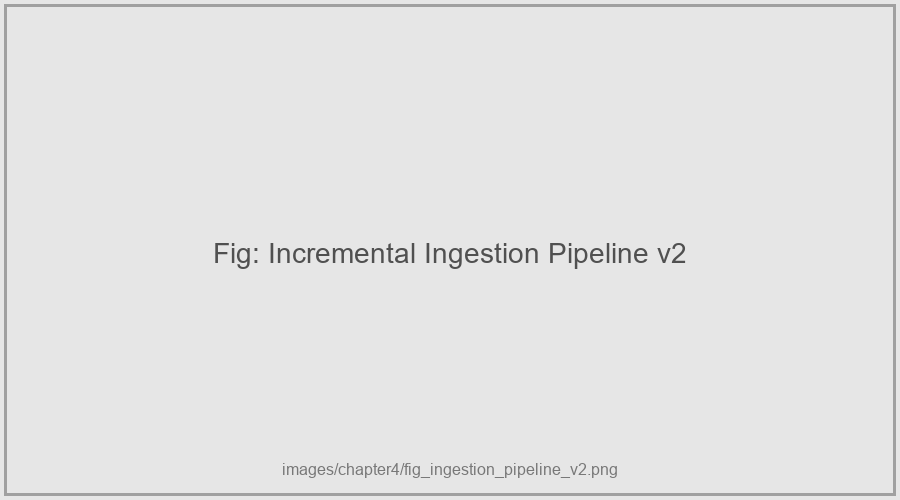
\includegraphics[width=0.90\textwidth]{images/chapter4/fig_ingestion_pipeline_v2}
\caption{Updated data ingestion pipeline. The incremental path (shaded) runs automatically when the background worker has drained 50 new interactions from Redis. Each stage is fault-isolated; a failure at any point retains the previous embeddings without interrupting the recommendation service.}
\label{fig:ingestion_pipeline_v2}
\end{figure}

\paragraph{Stage 1 — Delta export —}
The \texttt{export\_delta\_hyperedges.py} script queries the MongoDB \texttt{interactions} collection for all click and cart events recorded after the timestamp stored in \texttt{data/delta\_last\_run.txt}, defaulting to seven days prior if the file is absent.
Guest sessions (\texttt{is\_guest: true}) are excluded so that transient, unauthenticated activity does not corrupt the co-purchase graph.
For each qualifying user, the collected ASINs are accumulated into a Python \texttt{set}, which inherently deduplicates repeated clicks on the same item.
An ASIN whitelist loaded from \texttt{data/asins.csv} is applied as a catalogue boundary filter, ensuring consistency with the FAISS and metadata layers.
Each user's deduplicated item set is written as a single space-separated hyperedge line to \texttt{data/delta\_hyperedges.txt}.
On completion, the current timestamp is persisted to \texttt{delta\_last\_run.txt}; subsequent runs therefore query only new events, avoiding double-counting.
If no qualifying events are found, no delta file is written and the pipeline halts gracefully.

\paragraph{Stage 2 — Cleora augmentation —}
When a non-empty delta file is present, \texttt{run\_cleora.py --augment} is invoked as an asynchronous subprocess.
It ingests the delta hyperedges into the existing co-purchase graph and applies Markov-chain propagation to produce updated entity embeddings, writing the result to \texttt{data/cleora\_embeddings.npz}.

\paragraph{Stage 3 — Hot-reload —}
After the augmentation subprocess exits successfully, the updated NPZ file is loaded and passed to \texttt{Retriever.reload\_cleora()}.
This method atomically replaces the in-memory Cleora FAISS index and ASIN lookup table in a single Python assignment with no \texttt{await} points, so concurrent in-flight recommendation requests observe either the old index or the new one in full — never a partial state.

\subsection{Automated Triggering and Error Recovery}
\label{sec:cleora_trigger}

The three-stage pipeline is driven by the background \texttt{\_log\_worker} coroutine described in Section~\ref{sec:storage_analysis}.
The worker increments a counter each time it drains an entry from the Redis queue into MongoDB.
When the counter reaches \texttt{CLEORA\_REFIT\_THRESHOLD} (default 50, overridable via environment variable), the full refit pipeline is launched as a non-blocking \texttt{asyncio.create\_task}.
An \texttt{asyncio.Event} gate prevents concurrent refits: if the threshold is crossed again while a refit is in progress, the event is ignored until the running task releases the gate.

Error recovery is implemented independently at each stage.
If the delta export subprocess exits with a non-zero return code, the pipeline is aborted before any file is written.
If the Cleora augmentation fails, the existing \texttt{cleora\_embeddings.npz} is left untouched.
If the hot-reload call raises an exception, the failure is logged and the previous in-memory index continues to serve requests.
This three-level isolation ensures that a partial failure leaves the system in a degraded-but-functional state rather than an inconsistent one, with no manual cleanup required.
